\documentclass[9pt,a5paper,]{book}
\usepackage{lmodern}
\usepackage{amssymb,amsmath}
\usepackage{ifxetex,ifluatex}
\usepackage{fixltx2e} % provides \textsubscript
\ifnum 0\ifxetex 1\fi\ifluatex 1\fi=0 % if pdftex
  \usepackage[T1]{fontenc}
  \usepackage[utf8]{inputenc}
\else % if luatex or xelatex
  \ifxetex
    \usepackage{mathspec}
  \else
    \usepackage{fontspec}
  \fi
  \defaultfontfeatures{Ligatures=TeX,Scale=MatchLowercase}
\fi
% use upquote if available, for straight quotes in verbatim environments
\IfFileExists{upquote.sty}{\usepackage{upquote}}{}
% use microtype if available
\IfFileExists{microtype.sty}{%
\usepackage{microtype}
\UseMicrotypeSet[protrusion]{basicmath} % disable protrusion for tt fonts
}{}
\usepackage[left=2cm,right=1.2cm,top=1.5cm,bottom=1.5cm]{geometry}
\usepackage{hyperref}
\hypersetup{unicode=true,
            pdftitle={Regression Models for Count Data: beyond the Poisson model},
            pdfauthor={Wagner Hugo Bonat; Walmes Marques Zeviani; Eduardo Elias Ribeiro Jr},
            pdfborder={0 0 0},
            breaklinks=true}
\urlstyle{same}  % don't use monospace font for urls
\usepackage{natbib}
\bibliographystyle{apalike}
\usepackage{color}
\usepackage{fancyvrb}
\newcommand{\VerbBar}{|}
\newcommand{\VERB}{\Verb[commandchars=\\\{\}]}
\DefineVerbatimEnvironment{Highlighting}{Verbatim}{commandchars=\\\{\}}
% Add ',fontsize=\small' for more characters per line
\newenvironment{Shaded}{}{}
\newcommand{\KeywordTok}[1]{\textbf{{#1}}}
\newcommand{\DataTypeTok}[1]{\underline{{#1}}}
\newcommand{\DecValTok}[1]{{#1}}
\newcommand{\BaseNTok}[1]{{#1}}
\newcommand{\FloatTok}[1]{{#1}}
\newcommand{\ConstantTok}[1]{{#1}}
\newcommand{\CharTok}[1]{{#1}}
\newcommand{\SpecialCharTok}[1]{{#1}}
\newcommand{\StringTok}[1]{{#1}}
\newcommand{\VerbatimStringTok}[1]{{#1}}
\newcommand{\SpecialStringTok}[1]{{#1}}
\newcommand{\ImportTok}[1]{{#1}}
\newcommand{\CommentTok}[1]{\textit{{#1}}}
\newcommand{\DocumentationTok}[1]{\textit{{#1}}}
\newcommand{\AnnotationTok}[1]{\textit{{#1}}}
\newcommand{\CommentVarTok}[1]{\textit{{#1}}}
\newcommand{\OtherTok}[1]{{#1}}
\newcommand{\FunctionTok}[1]{{#1}}
\newcommand{\VariableTok}[1]{{#1}}
\newcommand{\ControlFlowTok}[1]{\textbf{{#1}}}
\newcommand{\OperatorTok}[1]{{#1}}
\newcommand{\BuiltInTok}[1]{{#1}}
\newcommand{\ExtensionTok}[1]{{#1}}
\newcommand{\PreprocessorTok}[1]{\textbf{{#1}}}
\newcommand{\AttributeTok}[1]{{#1}}
\newcommand{\RegionMarkerTok}[1]{{#1}}
\newcommand{\InformationTok}[1]{\textit{{#1}}}
\newcommand{\WarningTok}[1]{\textit{{#1}}}
\newcommand{\AlertTok}[1]{\textbf{{#1}}}
\newcommand{\ErrorTok}[1]{\textbf{{#1}}}
\newcommand{\NormalTok}[1]{{#1}}
\usepackage{longtable,booktabs}
\usepackage{graphicx,grffile}
\makeatletter
\def\maxwidth{\ifdim\Gin@nat@width>\linewidth\linewidth\else\Gin@nat@width\fi}
\def\maxheight{\ifdim\Gin@nat@height>\textheight\textheight\else\Gin@nat@height\fi}
\makeatother
% Scale images if necessary, so that they will not overflow the page
% margins by default, and it is still possible to overwrite the defaults
% using explicit options in \includegraphics[width, height, ...]{}
\setkeys{Gin}{width=\maxwidth,height=\maxheight,keepaspectratio}
\IfFileExists{parskip.sty}{%
\usepackage{parskip}
}{% else
\setlength{\parindent}{0pt}
\setlength{\parskip}{6pt plus 2pt minus 1pt}
}
\setlength{\emergencystretch}{3em}  % prevent overfull lines
\providecommand{\tightlist}{%
  \setlength{\itemsep}{0pt}\setlength{\parskip}{0pt}}
\setcounter{secnumdepth}{5}
% Redefines (sub)paragraphs to behave more like sections
\ifx\paragraph\undefined\else
\let\oldparagraph\paragraph
\renewcommand{\paragraph}[1]{\oldparagraph{#1}\mbox{}}
\fi
\ifx\subparagraph\undefined\else
\let\oldsubparagraph\subparagraph
\renewcommand{\subparagraph}[1]{\oldsubparagraph{#1}\mbox{}}
\fi

%%% Use protect on footnotes to avoid problems with footnotes in titles
\let\rmarkdownfootnote\footnote%
\def\footnote{\protect\rmarkdownfootnote}

%%% Change title format to be more compact
\usepackage{titling}

% Create subtitle command for use in maketitle
\newcommand{\subtitle}[1]{
  \posttitle{
    \begin{center}\large#1\end{center}
    }
}

\setlength{\droptitle}{-2em}
  \title{Regression Models for Count Data: beyond the Poisson model}
  \pretitle{\vspace{\droptitle}\centering\huge}
  \posttitle{\par}
  \author{Wagner Hugo Bonat \\ Walmes Marques Zeviani \\ Eduardo Elias Ribeiro Jr}
  \preauthor{\centering\large\emph}
  \postauthor{\par}
  \date{}
  \predate{}\postdate{}

% Mathematics environments
\usepackage{amssymb}
\usepackage{amsmath}
\usepackage{amstext}
\usepackage{amsfonts}

% Figures
\usepackage{graphics}
\usepackage{natbib}

% Customize itemize's enviroments
\usepackage{enumitem}

% Fonts
\usepackage{mathpazo}
\usepackage{eulervm}
\usepackage{inconsolata}
\urlstyle{tt}

% Compact toc
\usepackage{tocloft}

% Footers and headers styles
\usepackage{fancyhdr}
\pagestyle{fancy}
\fancyhf{}
\fancyhead[LE,RO]{\thepage}
\fancyhead[RE]{\scriptsize\leftmark}
\fancyhead[LO]{\scriptsize\rightmark}

% Modify color in Rcodes/chunks (works well only monochrome highlight)
\usepackage{xcolor}
\definecolor{inputcolor}{RGB}{25,25,112}
\usepackage{framed}
\usepackage{fancyvrb}
\DefineVerbatimEnvironment{Highlighting}{Verbatim}{commandchars=\\\{\},
                                                   fontsize=\small}
\definecolor{shadecolor}{RGB}{248,248,248}
\renewenvironment{Shaded}{\color{inputcolor}}{}
\renewcommand{\DataTypeTok}[1]{{#1}}

% Modify style of verbatim (chunks outputs)
\definecolor{outputcolor}{RGB}{139,0,0}
\makeatletter
\def\verbatim@font{\ttfamily \small \color{outputcolor}}%
\makeatother

\usepackage{amsthm}
\newtheorem{theorem}{Theorem}[chapter]
\newtheorem{lemma}{Lemma}[chapter]
\theoremstyle{definition}
\newtheorem{definition}{Definition}[chapter]
\newtheorem{corollary}{Corollary}[chapter]
\newtheorem{proposition}{Proposition}[chapter]
\theoremstyle{definition}
\newtheorem{example}{Example}[chapter]
\theoremstyle{remark}
\newtheorem*{remark}{Remark}
\begin{document}
\maketitle

\thispagestyle{empty}
\cleardoublepage
\thispagestyle{empty}

\topskip0pt

\begin{flushleft}
  \Large \bf
  Regression Models for Count Data:\\
  beyond Poisson model
\end{flushleft}
\vspace*{1.5em}

\begin{flushleft}
Wagner Hugo Bonat\footnotemark[1] \footnotemark[3]\\
\url{www.leg.ufpr.br/~wagner}

Walmes Marques Zeviani\footnotemark[1] \footnotemark[3]\\
\url{www.leg.ufpr.br/~walmes}

Eduardo Elias Ribeiro Jr\footnotemark[2] \footnotemark[3]\\
\url{www.leg.ufpr.br/~eduardojr}
\end{flushleft}
\vspace*{2em}


\footnotemark[1]Departamento de Estatística (DEST)\\
\hspace*{1.5mm}Universidade Federal do Paraná (UFPR)

\footnotemark[2]Departamento de Ciências Exatas (LCE)\\
\hspace*{1.5mm}ESALQ - Universidade de São Paulo (ESALQ-USP)

\footnotemark[3]Laboratório de Estatística e Geoinformação (LEG)\\
\hspace*{1.5mm}\url{http://www.leg.ufpr.br}\\

Supplementary content: \url{http://www.leg.ufpr.br/rmcd}\\
Contact: \url{rmcd@leg.ufpr.br}
\vspace*{\fill}

\begin{center}
XV EMR - Escola de Modelos de Regressão\\
Goiânia - Goiás, Brasil\\
March 26 to 29, 2017
\end{center}

\clearpage
\thispagestyle{empty}
\pagebreak

\setcounter{page}{1}

{
\setcounter{tocdepth}{1}
\tableofcontents
}
\chapter*{Preface}\label{preface}
\addcontentsline{toc}{chapter}{Preface}

The main goal of this material is to provide a technical support for the
students attending the course ''Regression models for count data: beyond
the Poisson model``, given as part of the XV Brazilian School of
Regression models - March/2017 in Goiânia, Goiás, Brazil.

The main goal of this course is to present a wide range of statistical
models to deal with count data. We focus on parametric and second-moment
specified models. We shall present the model specification along with
strategies for model fitting and associated \texttt{R}\citep{R2015}
code. Furthermore, this book-course and supplementary materials as
\texttt{R} code and data sets are available for the students on the web
page \url{http://cursos.leg.ufpr.br/rmcd}.

We intend to keep the course in a level suitable for bachelor students
who already attended a course on generalized linear models
\citep{Nelder1972}. However, since the course also covers updated
topics, it can be of interest of postgraduate students and researches in
general.

We designed the course for three hours of tuition. In the first part
(two hours) of the course, we shall present the analysis of count data
based on fully parametric models. After a brief introduction and
motivation on count data, we present the Poisson, Gamma-Count,
Poisson-Tweedie and COM-Poisson distributions. We explore their
properties through a consideration of dispersion, zero-inflated and
heavy tail indexes. Furthermore, the estimation and inference for these
models based on the likelihood paradigm is discussed along with
\texttt{R} code and worked examples.

In the second part (one hour) of the course, we provide a brief
introduction to the estimating function approach \citetext{\citealp[
]{Jorgensen2004}; \citealp{Bonat2016a}} and discuss models based on
second-moment assumptions in the style of \citet{Wedderburn1974}. In
particular, we focus on the recently proposed Extended Poisson-Tweedie
model \citep{Bonat2016b} and its special case the quasi-Poisson model.
The estimating function approach adopted for estimation and inference is
presented along with \texttt{R} code and data examples. The use of the
\texttt{R} package \texttt{mcglm} \citep{Bonat2016c} is discussed for
fitting the extended Poisson-Tweedie model.

We acknowledge our gratitude to the scientific committee of XV Brazilian
regression model school for this opportunity.

Department of Statistics, Paraná Federal University, Curitiba, PR,
Brazil.

March 27, 2017.

\chapter{Introduction}\label{introduction}

The analysis of count data has received attention from the statistical
community in the last four decades. Since the seminal paper published by
Nelder and Wedderburn \citep{Nelder1972}, the class of generalized
linear models (GLMs) have a proeminent role for regression modelling of
normal and non-normal data. GLMs are fitted by a simple and efficient
Newton score algorithm relying only on second-moment assumptions for
estimation and inference. Furthermore, the theoretical background for
GLMs is well established in the class of dispersion models
\citep{Jorgensen1987, Jorgensen1997} as a generalization of the
exponential family of distributions.

In spite of the flexibility of the GLM class, the Poisson distribution
is the only choice for the analysis of count data in this framework.
Thus, in practice there is probably an over-emphasis on the use of the
Poisson distribution for count data. A well known limitation of the
Poisson distribution is its mean and variance relationship, which
implies that the variance equals the mean, referred to as
equidispersion. In practice, however, count data can present other
features, namely underdispersion (mean \textgreater{} variance) and
overdispersion (mean \textless{} variance). There are many different
possible causes for departures from the equidispersion. Furthermore, in
practical data analysis a number of these could be involved.

One possible cause of under/overdispersion is departure from the Poisson
process. It is well known that the Poisson counts can be interpreted as
the number of events in a given time interval where the arrival's times
are exponential distributed. When this assumption is violated the
resulting counts can be under or overdispersed \citep{Zeviani2014}.
Another possibility and probably more frequent cause of overdispersion
is unobserved heterogeneity of experimental units. It can be due, for
example, to correlation between individual responses, cluster sampling,
ommitted covariates and others.

In general, these departures from the Poisson distribution are
manifested in the raw data as a zero-inflated or heavy-tailed count
distribution. It is important to discuss the consequences of failing to
take into account the under or overdispersion when analysing count data.
In the case of overdispersion, the standard errors associated with the
regression coefficients calculated under the Poisson assumption are too
optimistic and associated hypothesis tests will tend to give false
positive results by incorrectly rejecting null hypotheses. The opposite
situation will appear in case of underdispersed data. In both cases, the
Poisson model provides unreliable standard errors for the regression
coefficients and hence potentially misleading inferences. However, the
regression coefficients are still consistently estimated.

The strategies for constructing alternative count distributions are
related with the causes of the non-equidispersion. When departures from
the Poisson process are plausible the class of duration dependence
models \citep{Winkelmann2003} can be employed. This class of models
changes the distribution of the time between events from the exponential
to more general distributions, like gamma and inverse Gaussian. In this
course, we shall discuss one example of this approach, namely, the
Gamma-Count distribution \citep{Zeviani2014}. This distribution assumes
that the time between events is gamma distributed, thus it can deal with
under, equi and overdispersed count data.

On the other hand, if unobserved heterogeneity is present its in general
implies extra variability and consequently overdispersed count data. In
this case, a Poisson mixtures is commonly applied. This approach
consists of include random effects on the observation level, and thus
take into account the unobserved heterogeneity. Probably, the most
popular example of this approach is the negative binomial model, that
corresponds to a Poisson-gamma mixtures. In this course, we shall
present the Poisson-Tweedie family of distributions, which in turn
corresponds to Poisson-Tweedie mixtures
\citep{Bonat2016b, Jorgensen2014}. Finally, a third approach to deal
with non-equidispersed count data consists of generalize the Poisson
distribution by adding an extra parameter to model under and
overdispersion. Such a generalization can be done using the class of
weighted Poisson distributions \citep{DelCastillo1998}. One popular
example of this approach is the Conway--Maxwell--Poisson distribution
(COM-Poisson) \citep{Sellers2010}. The COM-Poisson is a member of the
exponential family, has the Poisson and geometric distributions as
special cases and the Bernoulli distribution as a limiting case. It can
deal with both under and overdispersed count data. Thus, given the nice
properties of the COM-Poisson distribution for handling count data, we
choose to present this model as part of this short course.

In this short course, we shall highlight and compare the ability of
these distributions to deal with count data through a consideration of
dispersion, zero-inflated and heavy tail indexes. Furthermore, we
specify regression models and illustrate their application with two
worked examples.

In Chapter \ref{models} we present the properties and regression models
associated with the Poisson, Gamma-count, Poisson-Tweedie and
COM-Poisson distributions. Furthermore, we compare these distributions
using the dispersion, zero-inflated and heavy-tail indexes. Estimation
and inference for these models based on the likelihood paradigm are
discussed in Chapter \ref{likelihood}. In Chapter \ref{SM}, we extend
the Poisson-Tweedie model using only second-moment assumptions and the
fitting algorithm based on the estimating functions approach. Chapter
\(5\) presents two worked examples. Finally, in Chapter \(6\) we discuss
the general methods and propose some topics for future works.

\chapter{Count distributions: properties and regression
models}\label{models}

In this chapter, we present the probability mass function and discuss
the main properties of the Poisson, Gamma-Count, Poisson-Tweedie and
COM-Poisson distributions.

\section{Poisson distribution}\label{poisson-distribution}

The Poisson distribution is a notorious discrete distribution. It has a
dual interpretation as a natural exponential family and as an
exponential dispersion model. The Poisson distribution denoted by
\(P(\mu)\) has probability mass function

\begin{eqnarray}
p(y;\mu) &=& \frac{\mu^y}{y!}\exp\{-\mu\} \\
         &=& \frac{1}{y!} \exp \{\phi y -  \exp\{\phi\} \}, \quad y \in \mathbb{N}_{0},
\label{eq:Poisson}
\end{eqnarray}

where \(\phi = \log \{\mu\} \in \mathbb{R}\). Hence the Poisson is a
natural exponential family with cumulant generator
\(\kappa(\phi) = \exp\{\phi\}\). We have
\(\mathrm{E}(Y) = \kappa^{\prime}(\phi) = \exp\{\phi\} = \mu\) and
\(\mathrm{var}(Y) = \kappa^{\prime \prime}(\phi) = \exp\{\phi\} = \mu\).
The probability mass function \eqref{eq:Poisson} can be evaluated in
\texttt{R} through the \texttt{dpois()} function.

In order to specify a regression model based on the Poisson
distribution, we consider a cross-section dataset, \((y_i, x_i)\),
\(i = 1,\ldots, n\), where \(y_i\)'s are iid realizations of \(Y_i\)
according to a Poisson distribution. The Poisson regression models is
defined by
\[Y_i \sim P(\mu_i), \quad  \text{with} \quad \mu_i = g^{-1}(\boldsymbol{x_i}^{\top} \boldsymbol{\beta}).\]
In this notation, \(\boldsymbol{x_i}\) and \(\boldsymbol{\beta}\) are
(\(q \times 1\)) vectors of known covariates and unknown regression
parameters, respectively. Moreover, \(g\) is a standard link function,
for which we adopt the logarithm link function, but potentially any
other suitable link function could be adopted.

\section{Gamma-Count distribution}\label{gammacount}

The Poisson distribution as presented in \eqref{eq:Poisson} follows
directly from the natural exponential family and thus fits in the
generalized linear models (GLMs) framework. Alternatively, the Poisson
distribution can be derived by assuming independent and exponentially
distributed times between events \citep{Zeviani2014}. This derivation
allows for a flexible framework to specify more general models to deal
with under and overdispersed count data.

As point out by \citet{Winkelmann2003} the distributions of the arrival
times determine the distribution of the number of events. Following
\citet{Winkelman1995}, let \({\tau_k, k \in \mathbb{N}}\) denote a
sequence of waiting times between the \((k-1)\)th and the \(k\)th
events. Then, the arrival time of the \(y\)th event is given by
\(\nu_y = \sum_{k = 1}^{y} \tau_k\), for \(y = 1, 2, \ldots\).
Furthermore, denote \(Y\) the total number of events in the open
interval between \(0\) and \(T\). For fixed \(T\), \(Y\) is a count
variable. Indeed, from the definitions of \(Y\) and \(\nu_y\) we have
that \(Y < y\) iff \(\nu_y \ge T\), which in turn implies
\(P(Y < y) = P(\nu_y \ge T) = 1 - F_y(T)\), where \(F_y(T)\) denotes the
cumulative distribution function of \(\nu_y\). Furthermore,

\begin{eqnarray}
P(Y = y) &=& P(Y < y+1) - P(Y < y) \\
     &=& F_y(T) - F_{y+1}(T).
\label{eq:DURATION}
\end{eqnarray}

Equation \eqref{eq:DURATION} provides the fundamental relation between the
distribution of arrival times and the distribution of counts. Moreover,
this type of specification allows to derive a rich class of models for
count data by choosing a distribution for the arrival times. In this
material, we shall explore the Gamma-Count distribution which is
obtained by specifying the arrival times distribution as gamma
distributed.

Let \(\tau_k\) be identically and independently gamma distributed, with
density distribution (dropping the index \(k\)) given by

\begin{equation}
f(\tau; \alpha, \gamma) = \frac{\gamma^{\alpha}}{\Gamma(\alpha)} \tau^{\alpha-1} \exp\{-\gamma \tau\}, \quad \alpha, \gamma \in \mathbb{R}^{+}.
\end{equation}

In this parameterization \(\mathrm{E}(\tau) = \alpha/\gamma\) and
\(\mathrm{var}(\tau) = \alpha/\gamma^2\). Thus, by applying the
convolution formula for gamma distributions, it is easy to show that the
distribution of \(\nu_y\) is given by

\begin{equation}
f_y(\nu; \alpha, \gamma) = \frac{\gamma^{y\alpha}}{\Gamma(y\alpha)} \nu^{y\alpha-1} \exp\{-\gamma \nu\}.
\end{equation}

To derive the new count distribution, we have to evaluate the cumulative
distribution function, which after the change of variable
\(u = \gamma \alpha\) can be written as

\begin{equation}
F_y(T) = \frac{1}{\Gamma(y\alpha)} \int_0^{\gamma T} u^{n\alpha -1} \exp\{-u\} du,
\label{eq:INTEGRAL}
\end{equation}

where the integral is the incomplete gamma function. We denote the right
side of \eqref{eq:INTEGRAL} as \(G(\alpha y, \gamma T)\). Thus, the number
of event occurrences during the time interval \((0,T)\) has the
two-parameter distribution function

\begin{equation}
P(Y = y) = G(\alpha y, \gamma T) - G(\alpha (y + 1), \gamma T),
\label{eq:MASSFUNCTION}
\end{equation}

for \(y = 0, 1, \ldots\), where \(\alpha, \gamma \in \mathbb{R}^+\).
\citet{Winkelman1995} showed that for integer \(\alpha\) the probability
mass function defined in \eqref{eq:MASSFUNCTION} is given by

\begin{equation}
P(Y = y) = \exp^{\{-\gamma T\}} \sum_{i = 0}^{\alpha -1} \frac{(\gamma T)^{\alpha y + i}}{\alpha y + i}!.
\end{equation}

For \(\alpha = 1\), \(f(\tau)\) is the exponential distribution and
\eqref{eq:MASSFUNCTION} clearly simplifies to the Poisson distribution.
The following \texttt{R} function can be used to evaluate the
probability mass function of the Gamma-Count distribution.

\begin{Shaded}
\begin{Highlighting}[]
\NormalTok{dgc <-}\StringTok{ }\NormalTok{function(y, gamma, alpha, }\DataTypeTok{log =} \OtherTok{FALSE}\NormalTok{) \{}
  \NormalTok{p <-}\StringTok{ }\KeywordTok{pgamma}\NormalTok{(}\DataTypeTok{q =} \DecValTok{1}\NormalTok{,}
              \DataTypeTok{shape =} \NormalTok{y *}\StringTok{ }\NormalTok{alpha,}
              \DataTypeTok{rate =} \NormalTok{alpha *}\StringTok{ }\NormalTok{gamma) -}
\StringTok{    }\KeywordTok{pgamma}\NormalTok{(}\DataTypeTok{q =} \DecValTok{1}\NormalTok{,}
           \DataTypeTok{shape =} \NormalTok{(y +}\StringTok{ }\DecValTok{1}\NormalTok{) *}\StringTok{ }\NormalTok{alpha,}
           \DataTypeTok{rate =} \NormalTok{alpha *}\StringTok{ }\NormalTok{gamma)}
  \NormalTok{if(log ==}\StringTok{ }\OtherTok{TRUE}\NormalTok{) \{p <-}\StringTok{ }\KeywordTok{log}\NormalTok{(p)\}}
  \KeywordTok{return}\NormalTok{(p)}
\NormalTok{\}}
\end{Highlighting}
\end{Shaded}

Although, numerical evaluation of \eqref{eq:MASSFUNCTION} can easily be
done, the moments (mean and variance) cannot be obtained in closed form.
\citet{Winkelman1995} showed for a random variable
\(Y \sim GC(\alpha, \gamma)\), where \(GC(\alpha, \gamma)\) denotes a
Gamma-Count distribution with parameters \(\alpha\) and \(\gamma\),
\(\mathrm{E}(Y) = \sum_{i = 1}^\infty G(\alpha i, \gamma T)\).

Furthermore, for increasing \(T\) it holds that

\begin{equation}
Y(T) \overset{a}{\sim} N\left(\frac{\gamma T}{\alpha}, \frac{\gamma T}{\alpha^2} \right), 
\end{equation}

thus the limiting variance-mean ratio equals a constant \(1/\alpha\).
Consequently, the Gamma-Count distribution displays overdispersion for
\(0 < \alpha < 1\) and underdispersion for \(\alpha > 1\). Figure
\ref{fig:PlotGC} presents the probability mass function for some
Gamma-Count distributions. We fixed the parameter \(\gamma = 10\) and
fit the parameter \(\alpha\) in order to have dispersion index
(\(\mathrm{DI} = \mathrm{var}(Y)/\mathrm{E}(Y)\)) equaling to \(0.5\),
\(2\), \(5\) and \(20\).

\begin{figure}[h]

{\centering 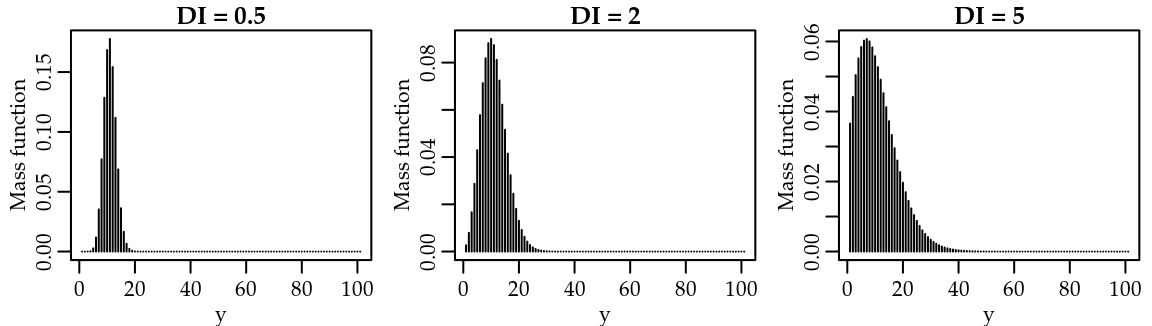
\includegraphics{rmcdbook_files/figure-latex/PlotGC-1} 

}

\caption{Gamma-Count probability mass function by values of the dispersion index (DI).}\label{fig:PlotGC}
\end{figure}

The Gamma-Count regression model assumes that the period at risk \((T)\)
is identical for all observations, thus \(T\) may be set to unity
without loss of generality. In the Gamma-count regression model, the
parameters depend on a vector of individual covariates
\(\boldsymbol{x}_i\). Thus, the Gamma-Count regression model is defined
by

\begin{equation}
\mathrm{E}(\tau_i | \boldsymbol{x}_i) = \frac{\alpha}{\gamma} = g^{-1}(-\boldsymbol{x_i}^\top \boldsymbol{\beta}).
\end{equation}

Consequently, the regression model is for the waiting times and not
directly for the counts. Note that,
\(\mathrm{E}(N_i | \boldsymbol{x}_i) = \mathrm{E}(\tau_i | \boldsymbol{x}_i)^{-1}\)
iff \(\alpha = 1\). Thus, \(\hat{\boldsymbol{\beta}}\) should be
interpreted accordingly. \(-\beta\) measures the percentage change in
the expected waiting time caused by a unit increase in \(x_i\). The
model parameters can be estimated using the maximum likelihood method as
we shall discuss in Chapter \ref{likelihood}.

\section{Poisson-Tweedie distribution}\label{ptw}

The Poisson-Tweedie distribution
\citep{Bonat2016b, Jorgensen2014, Shaarawi2011} consists of include
Tweedie distributed random effects on the observation level of Poisson
random variables, and thus to take into account unobserved
heterogeneity. The Poisson-Tweedie family is given by the following
hierarchical specification

\begin{eqnarray}
Y|Z &\sim& \mathrm{Poisson}(Z) \\ 
Z &\sim& \mathrm{Tw}_p(\mu, \phi), \nonumber
\label{eq:conditional}
\end{eqnarray}

where \(\mathrm{Tw}_p(\mu, \phi)\) denotes a Tweedie distribution
\citetext{\citealp[ ]{Jorgensen1987}; \citealp{Jorgensen1997}} with
probability function given by

\begin{equation}
f_{Z}(z; \mu, \phi, p) = a(z,\phi,p) \exp\{(z\psi - k_p(\psi))/\phi\}.
\label{eq:tweedie}
\end{equation}

In this notation, \(\mu = k^{\prime}_p(\psi)\) is the expectation,
\(\phi > 0\) is the dispersion parameter, \(\psi\) is the canonical
parameter and \(k_p(\psi)\) is the cumulant function. Furthermore,
\(\mathrm{var}(Z) = \phi V(\mu)\) where
\(V(\mu) = k^{\prime \prime}_p(\psi)\) is the variance function. Tweedie
densities are characterized by power variance functions of the form
\(V(\mu) = \mu^p\), where \(p \in (-\infty ,0] \cup [1,\infty)\) is an
index determining the distribution. The support of the distribution
depends on the value of the power parameter. For \(p \geq 2\),
\(1 < p < 2\) and \(p = 0\) the support corresponds to the positive,
non-negative and real values, respectively. In these cases
\(\mu \in \Omega\), where \(\Omega\) is the convex support (i.e.~the
interior of the closed convex hull of the corresponding distribution
support). Finally, for \(p < 0\) the support corresponds to the real
values, however the expectation \(\mu\) is positive. Here, we required
\(p \geq 1\), to make \(\mathrm{Tw}_p(\mu, \phi)\) non-negative.

The function \(a(z,\phi, p)\) cannot be written in a closed form apart
of the special cases corresponding to the Gaussian (\(p = 0\)), Poisson
(\(\phi = 1\) and \(p = 1\)), non-central gamma (\(p = 3/2\)), gamma
(\(p = 2\)) and inverse Gaussian (\(p = 3\)) distributions
\citep{Jorgensen1997}. The compound Poisson distribution is obtained
when \(1 < p < 2\). This distribution is suitable to deal with
non-negative data with probability mass at zero and highly right-skewed
\citep{Andersen2016}.

The Poisson-Tweedie is an overdispersed factorial dispersion model
\citep{Jorgensen2014} and its probability mass function for \(p > 1\) is
given by

\begin{equation}
f(y;\mu,\phi,p) = \int_0^\infty \frac{z^y \exp{-z}}{y!} a(z,\phi,p) \exp\{(z\psi - k_p(\psi))/\phi\} dz.
\label{eq:pmfPTW}
\end{equation}

The integral \eqref{eq:pmfPTW} has no closed-form apart of the special
case corresponding to the negative binomial distribution, obtained when
\(p = 2\), i.e.~a Poisson gamma mixture. In the case of \(p=1\), the
integral \eqref{eq:pmfPTW} is replaced by a sum and we have the Neyman
Type A distribution. Further special cases include the Hermite
\((p = 0)\), Poisson compound Poisson \((1 < p < 2)\), factorial
discrete positive stable \((p > 2)\) and Poisson-inverse Gaussian
\((p = 3)\) distributions \citetext{\citealp[
]{Jorgensen2014}; \citealp{Kokonendji2004}}.

In spite of other approaches to compute the probability mass function of
the Poisson-Tweedie distribution are available in the literature
\citetext{\citealp[ ]{Esnaola2013}; \citealp{Barabesi2016}}. In this
material, we opted to compute it by numerical evaluation of the integral
in \eqref{eq:pmfPTW} using the Monte Carlo method as implemented by the
following functions.

\begin{Shaded}
\begin{Highlighting}[]
\CommentTok{# Integrand Poisson X Tweedie distributions}
\NormalTok{integrand <-}\StringTok{ }\NormalTok{function(x, y, mu, phi, power) \{}
    \NormalTok{int =}\StringTok{ }\KeywordTok{dpois}\NormalTok{(y, }\DataTypeTok{lambda =} \NormalTok{x)*}\KeywordTok{dtweedie}\NormalTok{(x, }\DataTypeTok{mu =} \NormalTok{mu, }
                                        \DataTypeTok{phi =} \NormalTok{phi, }\DataTypeTok{power =} \NormalTok{power)}
    \KeywordTok{return}\NormalTok{(int)}
\NormalTok{\}}

\CommentTok{# Computing the pmf using Monte Carlo}
\NormalTok{dptw <-}\StringTok{ }\NormalTok{function(y, mu, phi, power, control_sample) \{}
    \NormalTok{pts <-}\StringTok{ }\NormalTok{control_sample$pts}
    \NormalTok{norma <-}\StringTok{ }\NormalTok{control_sample$norma}
    \NormalTok{integral <-}\StringTok{ }\KeywordTok{mean}\NormalTok{(}\KeywordTok{integrand}\NormalTok{(pts, }\DataTypeTok{y =} \NormalTok{y, }\DataTypeTok{mu =} \NormalTok{mu, }\DataTypeTok{phi =} \NormalTok{phi, }
                               \DataTypeTok{power =} \NormalTok{power)/norma)}
    \KeywordTok{return}\NormalTok{(integral)}
\NormalTok{\}}
\NormalTok{dptw <-}\StringTok{ }\KeywordTok{Vectorize}\NormalTok{(dptw, }\DataTypeTok{vectorize.args =} \StringTok{"y"}\NormalTok{)}
\end{Highlighting}
\end{Shaded}

When using the Monte Carlo method we need to specify a proposal
distribution, from which samples will be taken to compute the integral
as an expectation. In the Poisson-Tweedie case is sensible to use the
Tweedie distribution as proposal. Thus, in our function we use the
argument \texttt{control\_sample} to provide these values. The advantage
of this approach is that we need to simulate values once and we can
reuse them for all evaluations of the probability mass function, as
shown in the following code.

\begin{Shaded}
\begin{Highlighting}[]
\KeywordTok{require}\NormalTok{(tweedie)}
\KeywordTok{set.seed}\NormalTok{(}\DecValTok{123}\NormalTok{)}
\NormalTok{pts <-}\StringTok{ }\KeywordTok{rtweedie}\NormalTok{(}\DataTypeTok{n =} \DecValTok{1000}\NormalTok{, }\DataTypeTok{mu =} \DecValTok{10}\NormalTok{, }\DataTypeTok{phi =} \DecValTok{1}\NormalTok{, }\DataTypeTok{power =} \DecValTok{2}\NormalTok{)}
\NormalTok{norma <-}\StringTok{ }\KeywordTok{dtweedie}\NormalTok{(pts, }\DataTypeTok{mu =} \DecValTok{10}\NormalTok{, }\DataTypeTok{phi =} \DecValTok{1}\NormalTok{, }\DataTypeTok{power =} \DecValTok{2}\NormalTok{)}
\NormalTok{control_sample <-}\StringTok{ }\KeywordTok{list}\NormalTok{(}\StringTok{"pts"} \NormalTok{=}\StringTok{ }\NormalTok{pts, }\StringTok{"norma"} \NormalTok{=}\StringTok{ }\NormalTok{norma) }
\KeywordTok{dptw}\NormalTok{(}\DataTypeTok{y =} \KeywordTok{c}\NormalTok{(}\DecValTok{0}\NormalTok{, }\DecValTok{5}\NormalTok{, }\DecValTok{10}\NormalTok{, }\DecValTok{15}\NormalTok{), }\DataTypeTok{mu =} \DecValTok{10}\NormalTok{, }\DataTypeTok{phi =} \DecValTok{1}\NormalTok{, }\DataTypeTok{power =} \DecValTok{2}\NormalTok{, }
     \DataTypeTok{control_sample =} \NormalTok{control_sample)}
\end{Highlighting}
\end{Shaded}

\begin{verbatim}
## [1] 0.0937 0.0590 0.0354 0.0217
\end{verbatim}

\begin{Shaded}
\begin{Highlighting}[]
\KeywordTok{dnbinom}\NormalTok{(}\DataTypeTok{x =} \KeywordTok{c}\NormalTok{(}\DecValTok{0}\NormalTok{, }\DecValTok{5}\NormalTok{, }\DecValTok{10}\NormalTok{, }\DecValTok{15}\NormalTok{), }\DataTypeTok{mu =} \DecValTok{10}\NormalTok{, }\DataTypeTok{size =} \DecValTok{1}\NormalTok{)}
\end{Highlighting}
\end{Shaded}

\begin{verbatim}
## [1] 0.0909 0.0564 0.0350 0.0218
\end{verbatim}

It is also possible to use the Gauss-Laguerre method to approximate the
integral in \eqref{eq:pmfPTW}. In the supplementary material
\texttt{Script2.R}, we provide \texttt{R} functions using both Monte
Carlo and Gauss-Laguerre methods to approximate the probability mass
function of Poisson-Tweedie distribution.

Figure \ref{fig:ptwpmfplot} presents the empirical probability mass
function of some Poisson-Tweedie distributions computed based on a
sample of size \(100000\) (gray). Furthermore, we present an
approximation (black) for the probability mass function obtained by
Monte Carlo integration. We considered different values of the Tweedie
power parameter \(p = 1.1\), \(2\), and \(3\) combined with different
values of the dispersion index. In all scenarios the expectation \(\mu\)
was fixed at \(10\).

\begin{figure}[h]

{\centering 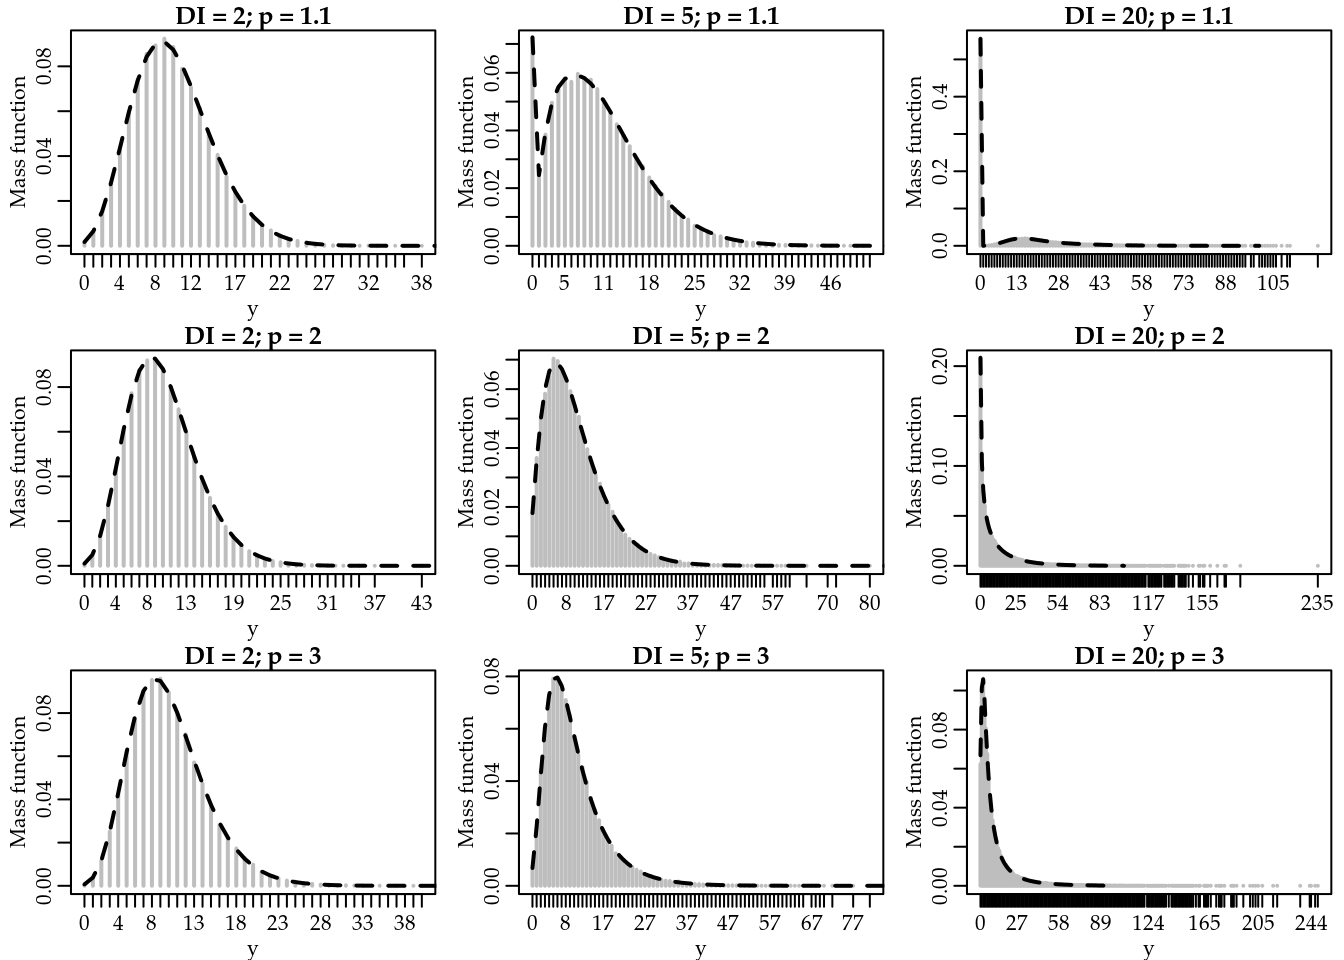
\includegraphics{rmcdbook_files/figure-latex/ptwpmfplot-1} 

}

\caption{Empirical (gray) and approximated (black) Poisson-Tweedie probability mass function by values of the dispersion index (DI) and Tweedie power parameter.}\label{fig:ptwpmfplot}
\end{figure}

For all scenarios considered the Monte Carlo method provides a quite
accurate approximation to the empirical probability mass function. For
these examples, we used \(5000\) random samples from the proposal
distribution.

Finally, the Poisson-Tweedie regression model is defined by
\[Y_i \sim PTw_{p}(\mu_i, \phi), \quad  \text{with} \quad \mu_i = g^{-1}(\boldsymbol{x_i}^{\top} \boldsymbol{\beta}),\]
where \(\boldsymbol{x}_i\) and \(\boldsymbol{\beta}\) are
\((q \times 1)\) vectors of known covariates and unknown regression
parameters. The estimation and inference of Poisson-Tweedie regression
models based on the maximum likelihood method are challenged by the
presence of an intractable integral in the probability mass function and
non-trivial restrictions on the power parameter space. In Chapter
\ref{likelihood}, we discuss maximum likelihood estimation for
Poisson-Tweedie regression. Furthermore, in Chapter \ref{SM} we extended
the Poisson-Tweedie model by using an estimating function approach in
the style of \citet{Wedderburn1974}.

\section{COM-Poisson distribution}\label{com-poisson-distribution}

The COM-Poisson distribution belongs to the family of weighted Poisson
distributions. A random variable \(Y\) is a weighted Poisson
distribution if its probability mass function can be written in the form

\[
f(y; \lambda, \nu) = \frac{\exp^{\{-\lambda\}} \lambda^y w_y}{W y!}, \quad y = 0, 1, \ldots,
\] where
\(W = \sum_{i = 0}^{\infty} \exp^{\{-\lambda\}} \lambda^i w_s / i!\) is
a normalizing constant \citep{Sellers2012}. The COM-Poisson is obtained
when \(w_{y} = (y!)^{1-\nu}\) for \(\nu \geq 0\). In general, the
expectation and variance of the COM-Poisson distribution cannot be
expressed in closed-form. However, they can be approximated by
\[\mathrm{E}(Y) \approx \lambda^{1/\nu} - \frac{\nu - 1}{2 \nu} \quad
\text{and} \quad \mathrm{var}(Y) \approx (1/ \nu) \lambda^{1 /\nu}.\]

These approximations are accurate when \(\nu \leq 1\) or
\(\lambda > 10^{\nu}\). The infinite sum involved in computing the
probability mass function of the COM-Poisson distribution can be
approximated to any level of precision. It can be evaluated in
\texttt{R} using the function \texttt{dcom()} from the
\texttt{compoisson} package \citep{Dunn2012}. Figure
\ref{fig:comPoispmfplot} presents some COM-Poisson probability mass
functions. We tried to find parameters \(\lambda\) and \(\nu\) in order
to have \(\mathrm{E}(Y) = 10\) and dispersion index equals to
\(\mathrm{DI} = 0.5, 2, 5\) and \(20\). However, we could not find any
parameter combination to have \(\mathrm{DI} = 20\).

\begin{figure}[h]

{\centering 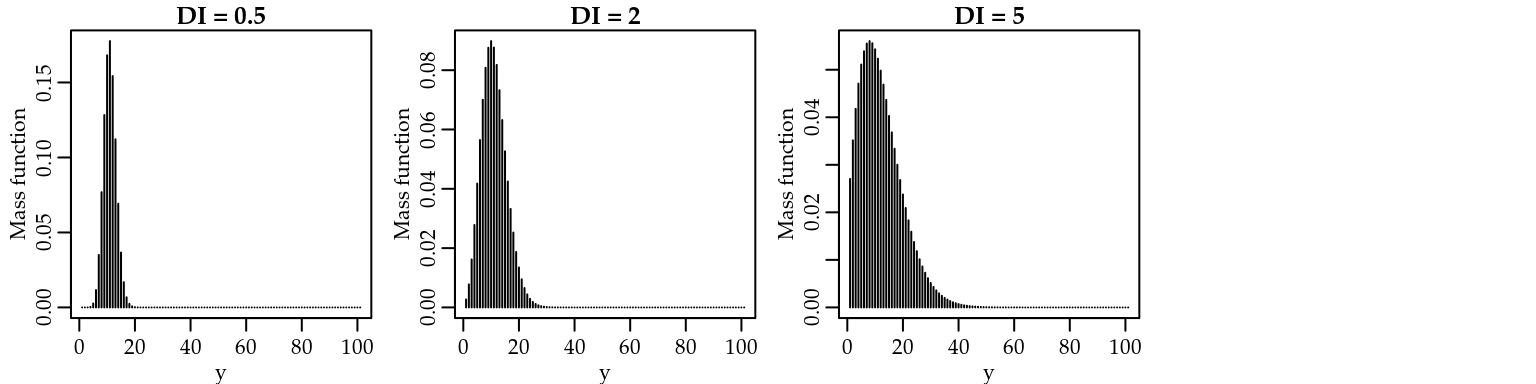
\includegraphics{rmcdbook_files/figure-latex/comPoispmfplot-1} 

}

\caption{COM-Poisson probability mass function by values of the dispersion index (DI).}\label{fig:comPoispmfplot}
\end{figure}

\citet{Sellers2010} proposed a regression model based on the COM-Poisson
distribution where the parameter \(\lambda\) is described by the values
of known covariates in a generalized linear models style. The
COM-Poisson regression model is defined by
\[Y_i \sim CP(\lambda_i, \nu), \quad  \text{with} \quad \lambda_i = g^{-1}(\boldsymbol{x_i}^{\top} \boldsymbol{\beta}).\]
In this notation, the parameter \(\nu\) is considered the dispersion
parameter such that \(\nu > 1\) represents underdispersion and
\(\nu < 1\) overdispersion. The Poisson model is obtained for
\(\nu = 0\) and as usual we adopt the logarithm link function for \(g\).

\section{Comparing count
distributions}\label{comparing-count-distributions}

Let \(Y\) be a count random variable and \(\mathrm{E}(Y) = \mu\) and
\(\mathrm{var}(Y)\) denote its mean and variance, respectively. To
explore and compare the flexibility of the models aforementioned, we
introduce the dispersion \((\mathrm{DI})\), zero-inflation
\((\mathrm{ZI})\) and heavy-tail \((\mathrm{HT})\) indexes, which are
respectively given by

\begin{equation}
\mathrm{DI} = \frac{\mathrm{var}(Y)}{\mathrm{E}(Y)}, \quad 
\mathrm{ZI} = 1 + \frac{\log \mathrm{P}(Y = 0)}{\mathrm{E}(Y)}
\end{equation}

and

\begin{equation}
\mathrm{HT} = \frac{\mathrm{P}(Y=y+1)}{\mathrm{P}(Y=y)}\quad \text{for} \quad y \to \infty. 
\end{equation}

These indexes are defined in relation to the Poisson distribution. Thus,
the dispersion index indicates underdispersion for \(\mathrm{DI} < 1\),
equidispersion for \(\mathrm{DI} = 1\) and overdispersion for
\(\mathrm{DI} > 1\). Similarly, the zero-inflated index is easily
interpreted, since \(\mathrm{ZI} < 0\) indicates zero-deflation,
\(\mathrm{ZI} = 0\) corresponds to no excess of zeroes and
\(\mathrm{ZI} > 0\) indicates zero-inflation. Finally,
\(\mathrm{HT} \to 1\) when \(y \to \infty\) indicates a heavy tail
distribution.

For the Poisson distribution the dispersion index equals \(1\)
\(\forall \mu\). In the Poisson case, it is easy to show that
\(\mathrm{ZI} = 0\) and \(\mathrm{HT} \to 0\) when \(y \to \infty\).
Thus, it is quite clear that the Poisson model can deal only with
equidispersed data and has no flexibility to deal with zero-inflation
and/or heavy tail count data. In fact, the presented indexes were
proposed in relation to the Poisson distribution in order to highlight
its limitations. Figure \ref{fig:indexes} presents the relationship
between mean and variance, the dispersion and zero-inflation indexes as
a function of the expected values \(\mu\) for different scenarios and
count distributions. Scenario \(1\) corresponds to the case of
underdispersion. Thus, we fixed the dispersion index at \(DI = 0.5\)
when the mean equaling \(10\). Since the Poisson-Tweedie cannot deal
with underdispersion, in this scenario we present only the Gamma-Count
and COM-Poisson distributions. Similarly, scenarios \(2--4\) are
obtained by fixing the dispesion index at \(DI = 2, 5\) and \(10\) when
mean equaling \(10\). In the scenario \(4\) we could not find a
parameter configuration in order to have a COM-Poisson distribution with
dispersion index equals \(20\). Consequently, we present results only
for the Gamma-Count and Poisson-Tweedie distributions. Furthermore,
Figure \ref{fig:heavytail} presents the heavy tail index for some
extreme values of the random variable \(Y\).

\begin{figure}[h]

{\centering 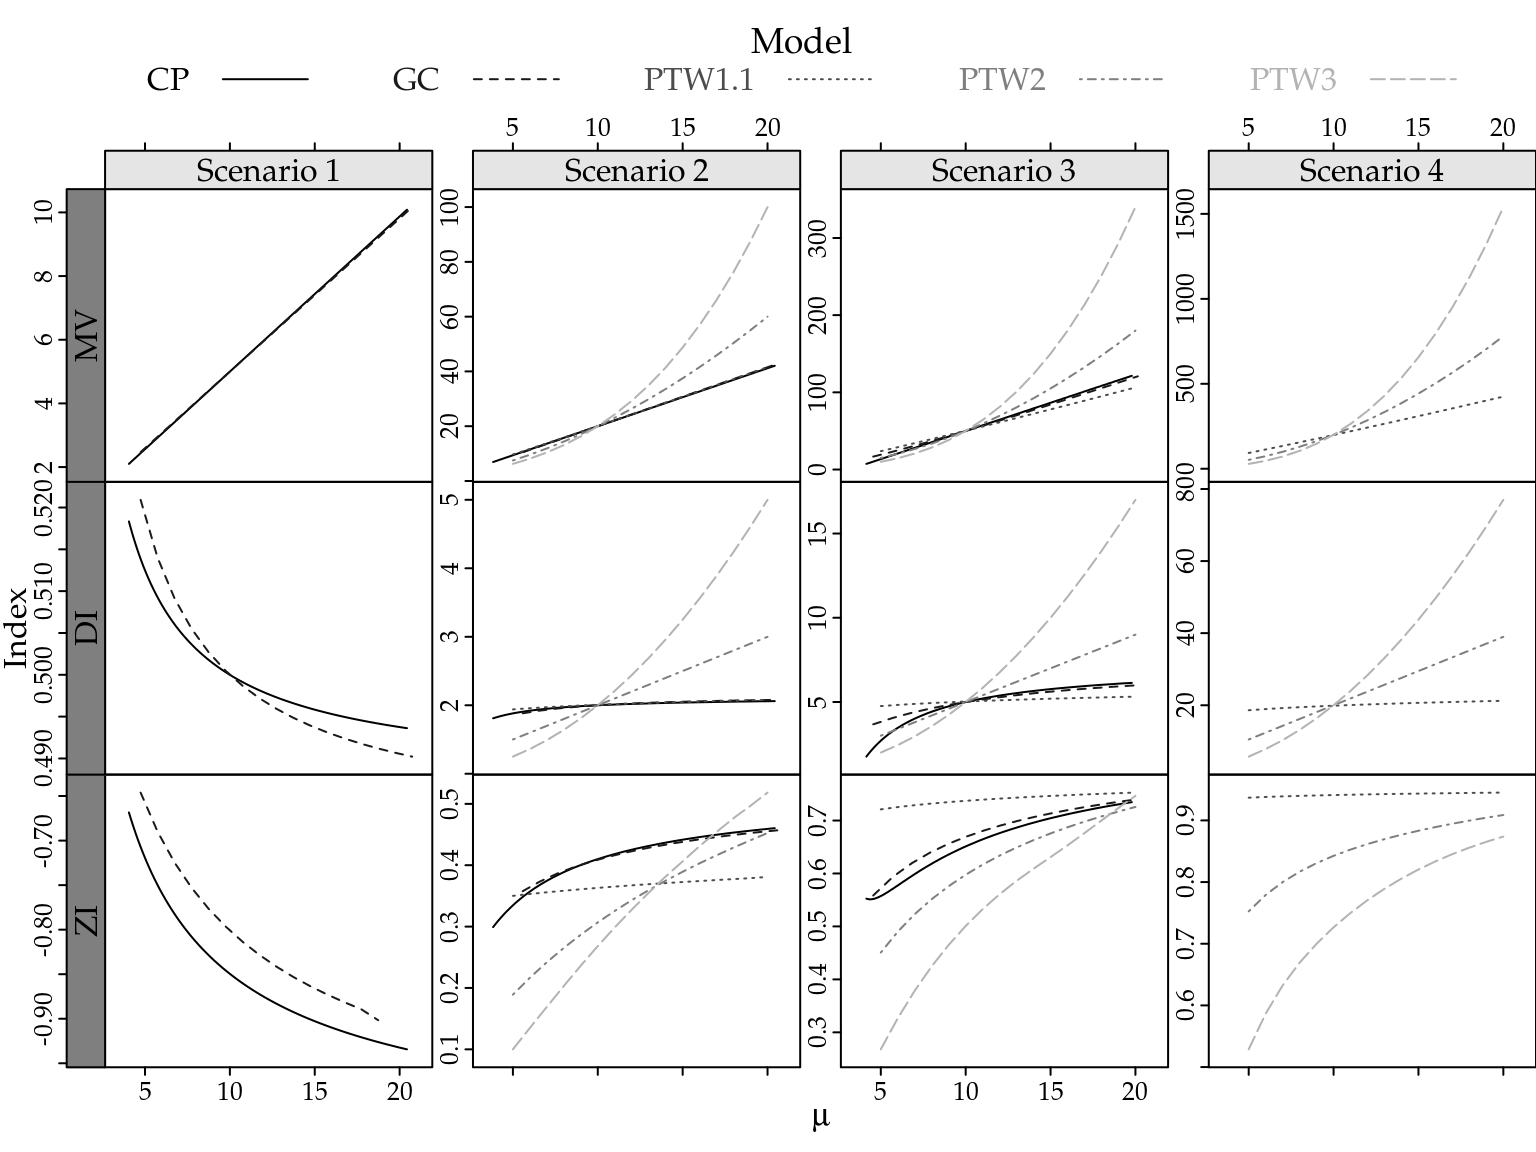
\includegraphics{rmcdbook_files/figure-latex/indexes-1} 

}

\caption{Mean and variance relationship (first line), dispersion (DI) and zero-inflation (ZI) indexes as a function of the expected values by simulation scenarios and count distributions.}\label{fig:indexes}
\end{figure}

\begin{figure}[h]

{\centering 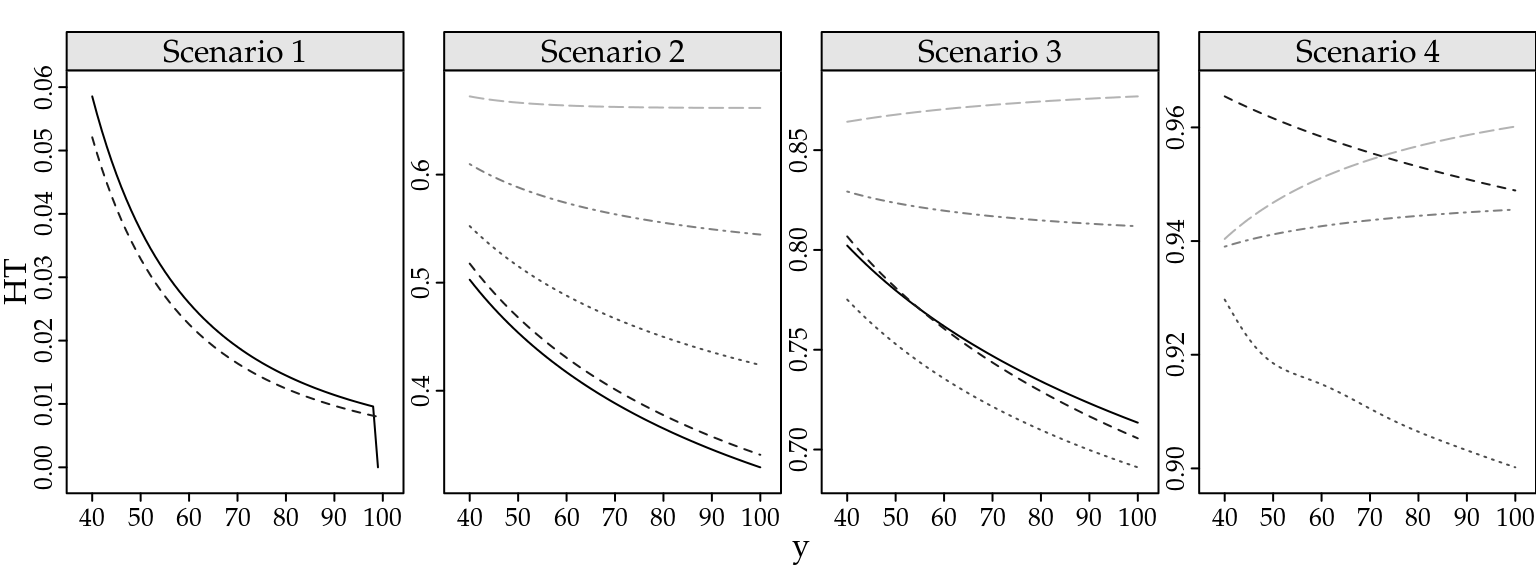
\includegraphics{rmcdbook_files/figure-latex/heavytail-1} 

}

\caption{Heavy tail index for some extreme values of the random variable Y by simulation scenarios and count distributions.}\label{fig:heavytail}
\end{figure}

The indexes presented in Figures \ref{fig:indexes} and
\ref{fig:heavytail} show that for all considered scenarios the
Gamma-Count and COM-Poisson distributions are quite similar. In general,
for these distributions, the indexes slightly depend on the expected
values and tend to stabilize for large values of \(\mu\). Consequently,
the mean and variance relationship is proportional to the dispersion
parameter value. In the overdispersion case, the Gamma-Count and
COM-Poisson distributions can handle with a limited ammount of
zero-inflation and are in general light tailed distributions, i.e.
\(\mathrm{HT} \to 0\) for \(y \to \infty\).

Regarding the Poisson-Tweedie distributions the indexes show that for
small values of the power parameter the Poisson-Tweedie distribution is
suitable to deal with zero-inflated count data. In that case, the
\(\mathrm{DI}\) and \(\mathrm{ZI}\) are almost not dependent on the
values of the mean. Furthermore, the \(\mathrm{HT}\) decreases as the
mean increases. On the other hand, for large values of the power
parameter the \(\mathrm{HT}\) increases with increasing mean, showing
that the model is specially suitable to deal with heavy tailed count
data. In this case, the \(\mathrm{DI}\) and \(\mathrm{ZI}\) increase
quickly as the mean increases giving an extremely overdispersed model
for large values of the mean. In general, the \(\mathrm{DI}\) and
\(\mathrm{ZI}\) are larger than one and zero, respectively, which, of
course, show that the corresponding Poisson-Tweedie distributions cannot
deal with underdispersed and zero-deflated count data.

In terms of regression models, the Poisson and Poisson-Tweedie models
are easy and convenient to interpret because the expected value is
directly modelled as a function of known covariates in a generalized
linear models manner. On the other hand, the Gamma-Count specifies the
regression model for the expectation of the times between events and,
thus requires careful interpretation. The COM-Poisson regression model
is hard to interpret and compare with the traditional Poisson regression
model, since it specifies the regression model for the parameter
\(\lambda\) that has no easy interpretation in relation to the
expectation of the count response variable.

Finally, in terms of computational implementation the simplicity of the
Poisson regression model is unquestionable. The probability mass
function of the Gamma-Count distribution requires the evaluation of the
difference between two cumulative gamma distributions. For large values
of the random variable \(Y\), such a difference can be time consuming
and inaccurately computed. Similarly, the COM-Poisson probability mass
function involves the evaluation of a infinity sum, which can be
computational expensive and inaccurate for large values of \(Y\).
Furthermore, for extreme values of \(\lambda\) and \(\nu\) the infinite
sum can numerically diverge making impossible to evaluate the
probability mass function. Finally, the Poisson-Tweedie probability mass
function involves an intractable integral, which makes the estimation
and inference based on likelihood methods computationally intensive.

\chapter{The method of maximum likelihood}\label{likelihood}

The estimation and inference for the models discussed in Chapter
\ref{models} can be done by the method of maximum likelihood
\citep{Silvey:1975}. In this Chapter, we present the maximum likelihood
method and its main properties along with some examples in \texttt{R}.
The maximum likelihood method is applicable mainly in situations where
the true distribution of the count random variable \(Y\) is known apart
of the values of a finite number of unknown parameters. Let
\(p(y;\boldsymbol{\theta})\) denote the true probability mass function
of the count random variable \(Y\). We assume that the family
\(p(y;\boldsymbol{\theta})\) is labelled by a (\(p \times 1\)) parameter
vector \(\boldsymbol{\theta}\) taking values in \(\Theta\) a subset of
\(\mathbb{R}^n\). For a given observed value \(y\) of the a random
variable \(Y\), the likelihood function corresponding to the observation
\(y\) is defined as
\(L(\boldsymbol{\theta};y) = p(y;\boldsymbol{\theta})\). It is important
to highlight that \(p(y;\boldsymbol{\theta})\) is a probability mass
function on the sample space. On the other hand,
\(L(\boldsymbol{\theta};y) = p(y;\boldsymbol{\theta})\) is a function on
the parameter space \(\Theta\). The likelihood function expresses the
plausibilities of different parameters after we have observed \(y\), in
the absence of any other information, we may have about these different
values. In particular, for count random variables the likelihood
function is the probability of the point \(y\) when
\(\boldsymbol{\theta}\) is the true parameter.

The method of maximum likelihood has a strong intuitive appeal and
according to it, we estimate the true parameter \(\boldsymbol{\theta}\)
by any parameter which maximizes the likelihood function. In general,
there is a unique maximizing parameter which is the most plausible and
this is the maximum likelihood estimate \citep{Silvey:1975}. In other
words, a maximum likelihood estimate \(\hat{\boldsymbol{\theta}}(y)\) is
any element of \(\Theta\) such that
\(L(\hat{\boldsymbol{\theta}}(y);y) = \underset{\boldsymbol{\theta}\in \Theta}\max L(\boldsymbol{\theta};y).\)
At this stage, we make the distinction between the estimate
\(\hat{\boldsymbol{\theta}}(y)\) and the estimator
\(\hat{\boldsymbol{\theta}}\). However, we are not maintain this
distinction and we shall use only \(\hat{\boldsymbol{\theta}}\) leaving
the context to make it clear whether we are thinking of
\(\hat{\boldsymbol{\theta}}\) as a function or as a particular value of
a function.

Let \(Y_i\) be independent and identically distributed count random
variables with probability mass function \(p(y;\boldsymbol{\theta})\),
whose observed values are denoted by \(y_i\) for \(i = 1, \ldots, n.\)
In this case, the likelihood function can be written as the product of
the individuals probability mass distributions, i.e.

\begin{equation}
L(\boldsymbol{\theta};\boldsymbol{y}) = \prod_{i=1}^n L(\boldsymbol{\theta}; y_i) = \prod_{i=1}^n p(y_i; \boldsymbol{\theta}).
\label{eq:LIK}
\end{equation}

For convenience, in practical situations is advisable to work with the
log-likelihood function obtained by taking the logarithm of Eq.
\eqref{eq:LIK}. Thus, the maximum likelihood estimator (MLE) for the
parameter vector \(\boldsymbol{\theta}\) is obtained by maximizing the
following log-likelihood function,

\begin{equation}
\ell(\boldsymbol{\theta})=\sum^n_{i=1} \log\{ L(\boldsymbol{\theta}; y_i) \}.
\label{eq:LOGLIK}
\end{equation}

Often, it is not possible to find a relatively simple expression in
closed form for the maximum likelihood estimates. However, it is usually
possible to assume that maximum likelihood estimates emerge as a
solution of the likelihood equations or also called score functions,
i.e.

\begin{equation}
\mathcal{U}(\boldsymbol{\theta}) = \left ( \frac{\partial \ell(\boldsymbol{\theta})}{\partial \theta_1}^\top, \ldots, \frac{\partial \ell(\boldsymbol{\theta})}{\partial \theta_p}^\top \right )^\top = \boldsymbol{0}.
\label{eq:SCORE}
\end{equation}

However, the system of non-linear equations in \eqref{eq:SCORE} often have
to be solved numerically. The entry \((i,j)\) of the \(p \times p\)
Fisher information matrix \(\mathcal{F}_{\boldsymbol{\theta}}\) for the
vector of parameter \(\boldsymbol{\theta}\) is given by

\begin{equation}
\mathcal{F}_{\boldsymbol{\theta}_{ij}} =-\mathrm{E} \left \{ \frac{\partial^2 \ell(\boldsymbol{\theta})}{\partial\theta_i\partial\theta_j} \right \}.
\end{equation}

In order to solve the system of equations
\(\mathcal{U}(\boldsymbol{\theta}) = \boldsymbol{0}\), we employ the
Newton scoring algorithm, defined by

\begin{eqnarray}
\boldsymbol{\theta}^{(i+1)} &=& \boldsymbol{\theta}^{(i)} - \mathcal{F}_{\boldsymbol{\theta}}^{-1} \mathcal{U}(\boldsymbol{\theta}^{(i)}). 
\end{eqnarray}

Finally, the well known distribution of the maximum likelihood estimator
\(\boldsymbol{\hat{\theta}}\) is
\(\mathrm{N}(\boldsymbol{\theta}, \mathcal{F}_{\boldsymbol{\theta}}^{-1})\).
Thus, the maximum likelihood estimator is asymptotically consistent,
unbiased and efficient.

A critical point of the approach described so far, is that we should be
able to compute the first and second derivatives of the log-likelihood
function. However, for the Gamma-Count where the log-likelihood function
is given by the difference between two integrals, we cannot obtain such
derivatives analytically. Similarly, for the COM-Poisson the
log-likelihood function involves an infinite sum and consequently such
derivatives cannot be obtained analitycally. Finally, in the
Poisson-Tweedie distribution the log-likelihood function is defined by
an intractable integral, which implies that we cannot obtain a
closed-form for the score function and Fisher information matrix.

Thus, an alternative approach is to maximize directly the log-likelihood
function in equation \eqref{eq:LOGLIK} using a derivative-free algorithm
as the Nelder-Mead method \citep{Nelder:1965} or some other numerical
method for maximizing the log-likelihood function, examples include the
\(BFGS\), conjugate gradient and simulated annealing. All of them are
implemented in \texttt{R} through the \texttt{optim()} function. The
package \texttt{bbmle} \citep{bbmle:2014} offers a suite of functions to
work with numerical maximization of log-likelihood functions in
\texttt{R}. As an example, consider the Gamma-Count distribution
described in subsection \ref{gammacount}. The log-likelihood function
for the parameters \(\theta = (\gamma, \alpha)\) in \texttt{R} is given
by

\begin{Shaded}
\begin{Highlighting}[]
\NormalTok{ll_gc <-}\StringTok{ }\NormalTok{function(gamma, alpha, y) \{}
  \NormalTok{ll <-}\StringTok{ }\KeywordTok{sum}\NormalTok{(}\KeywordTok{dgc}\NormalTok{(}\DataTypeTok{y =} \NormalTok{y, }\DataTypeTok{gamma =} \NormalTok{gamma, }\DataTypeTok{alpha =} \NormalTok{alpha, }\DataTypeTok{log =} \OtherTok{TRUE}\NormalTok{))}
  \KeywordTok{return}\NormalTok{(-ll)}
\NormalTok{\}}
\end{Highlighting}
\end{Shaded}

Thus, for a given vector of observed count values, we can numerically
maximize the log-likelihood function above using the function
\texttt{mle2()} from the \texttt{bbmle}package. It is important to
highlight that by default the \texttt{mle2()} function requires the
negative of the log-likelihood function instead of the log-likelihood
itself. Thus, our function returns the negative value of the
log-likelihood function.

\begin{Shaded}
\begin{Highlighting}[]
\KeywordTok{require}\NormalTok{(bbmle)}
\NormalTok{y <-}\StringTok{ }\KeywordTok{rpois}\NormalTok{(}\DecValTok{100}\NormalTok{, }\DataTypeTok{lambda =} \DecValTok{10}\NormalTok{)}
\NormalTok{fit_gc <-}\StringTok{ }\KeywordTok{mle2}\NormalTok{(ll_gc, }\DataTypeTok{start =} \KeywordTok{list}\NormalTok{(}\StringTok{"gamma"} \NormalTok{=}\StringTok{ }\DecValTok{10}\NormalTok{, }\StringTok{"alpha"} \NormalTok{=}\StringTok{ }\DecValTok{1}\NormalTok{), }
               \DataTypeTok{data =} \KeywordTok{list}\NormalTok{(}\StringTok{"y"} \NormalTok{=}\StringTok{ }\NormalTok{y))}
\end{Highlighting}
\end{Shaded}

The great advantage of the \texttt{bbmle} package for maximum likelihood
estimation in \texttt{R}, is that it already provides standard methods,
such as \texttt{summary()}, \texttt{coef()}, \texttt{confint()},
\texttt{vcov()}, \texttt{profile()} and other for objects of
\texttt{mle2} class.

\begin{Shaded}
\begin{Highlighting}[]
\KeywordTok{summary}\NormalTok{(fit_gc)}
\end{Highlighting}
\end{Shaded}

\begin{verbatim}
## Maximum likelihood estimation
## 
## Call:
## mle2(minuslogl = ll_gc, start = list(gamma = 10, alpha = 1), 
##     data = list(y = y))
## 
## Coefficients:
##       Estimate Std. Error z value   Pr(z)    
## gamma    9.842      0.335   29.38 < 2e-16 ***
## alpha    0.929      0.139    6.68 2.5e-11 ***
## ---
## Signif. codes:  0 '***' 0.001 '**' 0.01 '*' 0.05 '.' 0.1 ' ' 1
## 
## -2 log L: 518
\end{verbatim}

Similar functions can be done for the Poisson, Poisson-Tweedie and
COM-Poisson distributions. In the supplementary material
\texttt{Script5.R}, we provide some functions for maximum likelihood
estimation of Poisson-Tweedie and COM-Poisson distributions.

\chapter{Models specified by second-moment assumptions}\label{SM}

In Chapter \ref{models}, we presented four statistical models to deal
with count data and in the Chapter \ref{likelihood} the method of
maximum likelihood was introduced to estimate the model's parameters. As
discussed in Chapter \ref{likelihood} the method of maximum likelihood
assumes that the true distribution of the count random variable \(Y\) is
known apart of the values of a finite number of unknown parameters. In
this Chapter, we shall present a different approach for model
specification, estimation and inference based only on second-moment
assumptions.

\section{Extended Poisson-Tweedie
model}\label{extended-poisson-tweedie-model}

The Poisson-Tweedie distribution as presented in subsection the
\ref{ptw} provides a very flexible family of count distributions,
however, such a family has two main drawbacks: it cannot deal with
underdispersed count data and its probability mass function is given by
an intractable integral, which implies that estimation based on the
maximum likelihood method is computational demanding for practical data
analysis.

In spite of these issues \citep{Jorgensen2014} showed using factorial
cumulant function that for \(Y \sim PTw_p(\mu, \phi)\),
\(\mathrm{E}(Y) = \mu\) and \(\mathrm{var}(Y) = \mu + \phi \mu^p\). This
fact motivates \citep{Bonat2016b} to specify a model by using only
second-moment assumptions, i.e.~mean and variance.

Thus, consider a cross-section dataset, \((y_i, \boldsymbol{x}_i)\),
\(i = 1, \ldots, n\), where \(y_i\)'s are i.i.d. realizations of \(Y_i\)
according to an unspecified distribution, whose expectation and variance
are given by

\begin{align}
\mathrm{E}(Y_i) = \mu_i = g^{-1}(\boldsymbol{x}_i^{\top} \boldsymbol{\beta}) \\
\mathrm{var}(Y_i) = C_i = \mu_i + \phi \mu_i^p, 
\label{eq:EPTW}
\end{align}

where as before \(\boldsymbol{x}_i\) and \(\boldsymbol{\beta}\) are
(\(q \times 1\)) vectors of known covariates and unknown regression
parameters and \(g\) is the logarithm link function. The regression
model specified in (\ref{MODEL}) is parametrized by
\(\boldsymbol{\theta} = (\boldsymbol{\beta}^\top, \boldsymbol{\lambda}^\top )^\top\),
where \(\boldsymbol{\lambda} = (\phi, p)\).

Note that, based on second-moment assumptions, the only restriction to
have a proper model is that \(\mathrm{var}(Y_i) > 0\), thus
\[\phi > - \mu^{(1-p)}_i,\] which shows that at least at some extent
negative values for the dispersion parameter are allowed. Consequently,
the Poisson-Tweedie model can be extended to deal with underdispersed
count data, however, in doing so the associated probability mass
functions do not exist. However, in a regression modelling framework as
discussed in this material, we are in general interested in the
regression coefficient effects, thus such an issue does not imply any
loss of interpretation and applicability. The formulation of the
extended Poisson-Tweedie model is exactly the same of the quasi-binomial
and quasi-Poisson models popular in the context of generalized linear
models, see \citep[\citet{Nelder1972}]{Wedderburn1974} for details.
Furthermore, note that for \(p = 1\) the extended Poisson-Tweedie
regression model corresponds to a reparametrization of the popular
quasi-Poisson regression model.

It is also important to highlight that in this case the relationship
between mean and variance is proportional to the dispersion parameter
\(\phi\) as in the Gamma-Count and COM-Poisson distributions. Thus, we
expect for \(\phi < 0\) and \(p = 1\) the extended Poisson-Tweedie model
presents results in terms of regression coefficients really similar the
ones from the Gamma-Count and COM-Poisson regression models.

\section{Estimation and Inference}\label{estimation-and-inference}

Since the model presented in \eqref{eq:EPTW} is based only on
second-moment assumptions the method of maximum likelihood cannot be
employed. \citep{Bonat2016b} based on ideas of \citep{Jorgensen2004} and
\citep{Bonat2016a} proposed an estimating function approach for
estimation and inference for the extended Poisson-Tweedie regression
model. \citep{Bonat2016b} combined the quasi-score and Pearson
estimating functions for estimation of the regression and dispersion
parameters respectively. Following \citep{Bonat2016b} the quasi-score
function for \(\boldsymbol{\beta}\) has the following form,

\begin{equation*}
\psi_{\boldsymbol{\beta}}(\boldsymbol{\beta}, \boldsymbol{\lambda}) = \left (\sum_{i=1}^n \frac{\partial \mu_i}{\partial \beta_1}C^{-1}_i(Y_i - \mu_i), \ldots, \sum_{i=1}^n \frac{\partial \mu_i}{\partial \beta_q}C^{-1}_i(Y_i - \mu_i)  \right )^\top,
\end{equation*}

where \(\partial \mu_i/\partial \beta_j = \mu_i x_{ij}\) for
\(j = 1, \ldots, q\). The sensitivity matrix is defined as the
expectation of the first derivative of the estimating function with
respect to the model parameters. Thus, the entry \((j,k)\) of the
\(q \times q\) sensitivity matrix for \(\psi_{\boldsymbol{\beta}}\) is
given by

\begin{equation}
\mathrm{S}_{\boldsymbol{\beta}_{jk}} = \mathrm{E}\left ( \frac{\partial}{\partial \beta_k} \psi_{\boldsymbol{\beta}_j}(\boldsymbol{\beta}, \boldsymbol{\lambda})  \right ) = -\sum_{i=1}^n \mu_i x_{ij} C^{-1}_i x_{ik} \mu_i.
\label{eq:Sbeta}
\end{equation}

In a similar way, the variability matrix is defined as the variance of
the estimating function. In particular, for the quasi-score function the
entry \((j,k)\) of the \(q \times q\) variability matrix is given by

\begin{equation*}
\label{Vbeta}
\mathrm{V}_{\boldsymbol{\beta}_{jk}} = \mathrm{Cov}(\psi_{\boldsymbol{\beta}_j}(\boldsymbol{\beta}, \boldsymbol{\lambda}),\psi_{\boldsymbol{\beta}_k}(\boldsymbol{\beta}, \boldsymbol{\lambda})) = \sum_{i=1}^n \mu_i x_{ij} C^{-1}_i x_{ik} \mu_i.
\end{equation*}

The Pearson estimating function for the dispersion parameters has the
following form,

\begin{equation*}
\label{Pearson}
\psi_{\boldsymbol{\lambda}}(\boldsymbol{\lambda}, \boldsymbol{\beta}) = \left (-\sum_{i=1}^n \frac{\partial C^{-1}_i}{\partial \phi} \left [ (Y_i - \mu_i)^2 - C_i \right ], -\sum_{i=1}^n \frac{\partial C^{-1}_i}{\partial p}  \left [ (Y_i - \mu_i)^2 - C_i \right ]  \right )^\top.
\end{equation*}

Note that, the Pearson estimating functions are unbiased estimating
functions for \(\boldsymbol{\lambda}\) based on the squared residuals
\((Y_i - \mu_i)^2\) with expected value \(C_i\).

The entry \((j,k)\) of the \(2 \times 2\) sensitivity matrix for the
dispersion parameters is given by

\begin{equation}
\mathrm{S}_{\boldsymbol{\lambda}_{jk}} = \mathrm{E}\left ( \frac{\partial}{\partial \lambda_k}\psi_{\boldsymbol{\lambda}_j}(\boldsymbol{\lambda}, \boldsymbol{\beta})  \right ) = -\sum_{i=1}^n \frac{\partial C^{-1}_i}{\partial \lambda_j} C_i \frac{\partial C^{-1}_i}{\partial \lambda_k}C_i, 
\label{eq:Slambda}
\end{equation}

where \(\lambda_1\) and \(\lambda_2\) denote either \(\phi\) or \(p\).

Similarly, the cross entries of the sensitivity matrix are given by

\begin{equation}
\mathrm{S}_{\boldsymbol{\beta}_j \boldsymbol{\lambda}_k} = \mathrm{E}\left ( \frac{\partial}{\partial \lambda_k}\psi_{\boldsymbol{\beta}_j}(\boldsymbol{\beta}, \boldsymbol{\lambda})  \right ) = 0
\label{eq:Sbetalambda}
\end{equation}

and

\begin{equation}
\mathrm{S}_{\boldsymbol{\lambda}_j \boldsymbol{\beta}_k} = \mathrm{E}\left ( \frac{\partial}{\partial \beta_k}\psi_{\boldsymbol{\lambda}_j}(\boldsymbol{\lambda}, \boldsymbol{\beta})  \right ) = -\sum_{i=1}^n \frac{\partial C_i^{-1}}{\partial \lambda_j} C_i \frac{\partial C_i^{-1}}{\partial \beta_k} C_i.
\label{eq:Slambdabeta}
\end{equation}

Finally, the joint sensitivity matrix for the parameter vector
\(\boldsymbol{\theta}\) is given by

\begin{equation*}
\mathrm{S}_{\boldsymbol{\theta}} = \begin{pmatrix}
\mathrm{S}_{\boldsymbol{\beta}} & \boldsymbol{0} \\ 
\mathrm{S}_{\boldsymbol{\lambda}\boldsymbol{\beta}} & \mathrm{S}_{\boldsymbol{\lambda}}
\end{pmatrix},
\end{equation*}

whose entries are defined by equations \eqref{eq:Sbeta}, \eqref{eq:Slambda},
\eqref{eq:Sbetalambda} and \eqref{eq:Slambdabeta}.

We now calculate the asymptotic variance of the estimating function
estimators denoted by \(\boldsymbol{\hat{\theta}}\), as obtained from
the inverse Godambe information matrix, whose general form for a vector
of parameter \(\boldsymbol{\theta}\) is
\(\mathrm{J}^{-1}_{\boldsymbol{\theta}} = \mathrm{S}^{-1}_{\boldsymbol{\theta}} \mathrm{V}_{\boldsymbol{\theta}} \mathrm{S}^{-\top}_{\boldsymbol{\theta}}\),
where \(-\top\) denotes inverse transpose. The variability matrix for
\(\boldsymbol{\theta}\) has the form

\begin{equation}
\mathrm{V}_{\boldsymbol{\theta}} = \begin{pmatrix}
\mathrm{V}_{\boldsymbol{\beta}} & \mathrm{V}_{\boldsymbol{\beta}\boldsymbol{\lambda}} \\ 
\mathrm{V}_{\boldsymbol{\lambda}\boldsymbol{\beta}} & \mathrm{V}_{\boldsymbol{\lambda}}
\end{pmatrix},
\label{eq:VTHETA}
\end{equation}

where
\(\mathrm{V}_{\boldsymbol{\lambda}\boldsymbol{\beta}} = \mathrm{V}^{\top}_{\boldsymbol{\beta}\boldsymbol{\lambda}}\)
and \(\mathrm{V}_{\boldsymbol{\lambda}}\) depend on the third and fourth
moments of \(Y_i\), respectively. In order to avoid this dependence on
higher-order moments, we propose to use the empirical versions of
\(\mathrm{V}_{\boldsymbol{\lambda}}\) and
\(\mathrm{V}_{\boldsymbol{\lambda}\boldsymbol{\beta}}\) as given by

\begin{equation*}
\tilde{\mathrm{V}}_{\boldsymbol{\lambda}_{jk}} = \sum_{i=1}^n \psi_{\boldsymbol{\lambda}_j}(\boldsymbol{\lambda}, \boldsymbol{\beta})_i\psi_{\boldsymbol{\lambda}_k}(\boldsymbol{\lambda}, \boldsymbol{\beta})_i \quad \text{and} \quad \tilde{\mathrm{V}}_{\boldsymbol{\lambda}_j \boldsymbol{\beta}_k} = \sum_{i=1}^n \psi_{\boldsymbol{\lambda}_j}(\boldsymbol{\lambda}, \boldsymbol{\beta})_i \psi_{\boldsymbol{\beta}_k}(\boldsymbol{\lambda}, \boldsymbol{\beta})_i.
\end{equation*}

Finally, the well known asymptotic distribution of
\(\boldsymbol{\hat{\theta}}\) \citep{Jorgensen2004} is given by

\begin{equation*}
\boldsymbol{\hat{\theta}} \sim \mathrm{N}(\boldsymbol{\theta}, \mathrm{J}_{\boldsymbol{\theta}}^{-1}), \quad \text{where} \quad
\mathrm{J}^{-1}_{\boldsymbol{\theta}} = \mathrm{S}^{-1}_{\boldsymbol{\theta}} \mathrm{V}_{\boldsymbol{\theta}} \mathrm{S}^{-\top}_{\boldsymbol{\theta}}.
\end{equation*}

To solve the system of equations
\(\psi_{\boldsymbol{\beta}} = \boldsymbol{0}\) and
\(\psi_{\boldsymbol{\lambda}} = \boldsymbol{0}\) \citep{Jorgensen2004}
proposed the modified chaser algorithm, defined by

\begin{eqnarray*}
\label{chaser}
\boldsymbol{\beta}^{(i+1)} &=& \boldsymbol{\beta}^{(i)} - \mathrm{S}_{\boldsymbol{\beta}}^{-1} \psi_{\boldsymbol{\beta}}(\boldsymbol{\beta}^{(i)}, \boldsymbol{\lambda}^{(i)}) \nonumber \\
\boldsymbol{\lambda}^{(i+1)} &=& \boldsymbol{\lambda}^{(i)} - \alpha \mathrm{S}_{\boldsymbol{\lambda}}^{-1} \psi_{\boldsymbol{\lambda}}(\boldsymbol{\beta}^{(i+1)}, \boldsymbol{\lambda}^{(i)}).
\end{eqnarray*}

The modified chaser algorithm uses the insensitivity property
\eqref{eq:Sbetalambda}, which allows us to use two separate equations to
update \(\boldsymbol{\beta}\) and \(\boldsymbol{\lambda}\). We introduce
the tuning constant, \(\alpha\), to control the step-length. This
algorithm is a special case of the flexible algorithm presented by
\citet{Bonat2016a} in the context of multivariate covariance generalized
linear models. Hence, estimation for the extended Poisson-Tweedie model
is easily implemented in \texttt{R} through the \texttt{mcglm}
\citep{Bonat2016c} package.

\bibliography{config/rmcd.bib}


\end{document}
